\section{ResNet}\label{sect:resnet}
As said before, we are going to combine both the architectures of ResNets and Transformers. While we have covered most of the concepts of the Transformers, we are still lacking the necessary concepts about ResNets. Let us start with the input of this architecture: an image $X\in\mathbb{R}^{C\times H \times W}$, where $C$ represents the number of channels, $H$ represents the image height and $W$ represents the image width.

The input image will go through a series of convolutional blocks. Each convolutional block is shown in Fig.~\ref{fig:convblock}. As you can see, the input (a tensor of dimension $C\times H \times W$) goes through convolutional layers an activation layer, and normalization layers. After this, the tensor is summed with the input and another activation is applied. One of the most important things to note is the skip connection named \texttt{id}. This type of connection, discovered to be effective by \cite{He16}, is responsible for improving performance, reduce the vanishing/exploding gradient problem, and smoothing the loss landscape \cite{Li17}. Following this simple structure, usually, a max-pooling layer is applied to reduce the number of features per channel. 

A full depiction of a resnet architecture is shown in Fig.~\ref{fig:resnet}. As you can see, many convolutional blocks are applied one after another increasing the number of channels from the original number (usually 3) to 512. The final depicted block is responsible for outputting the classification. 

\begin{figure}
    \begin{subfigure}{.61\textwidth}
        \centering
        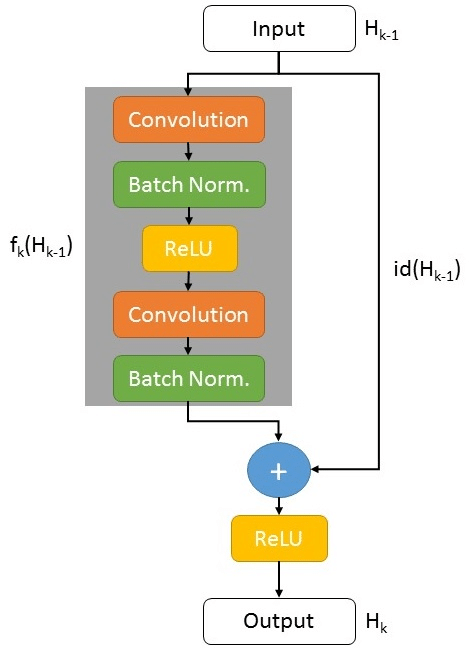
\includegraphics[width=.8\linewidth]{figs/convblock.png}
        \subcaption{Depiction of a convolutional block from \cite{Kumra17}}
        \label{fig:convblock}
    \end{subfigure}
    \begin{subfigure}{.5\textwidth}
        \centering
        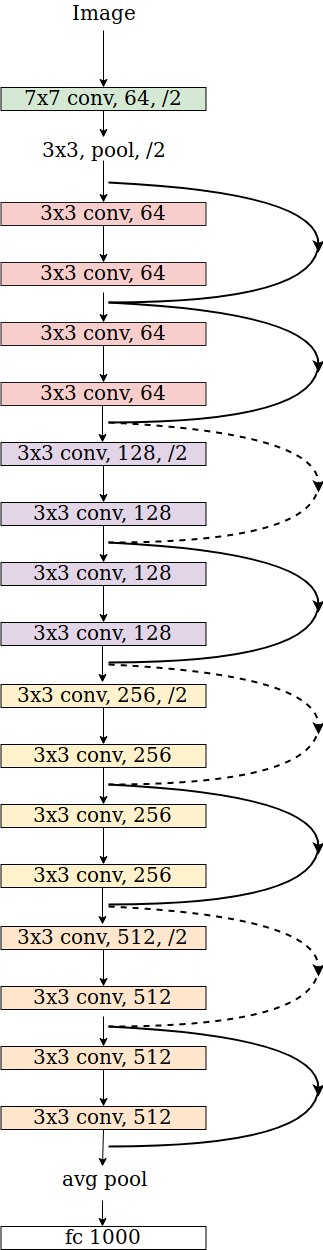
\includegraphics[width=.35\linewidth]{figs/resnet.png}
        \subcaption{Depiction of a ResNet from \cite{He16}}
        \label{fig:resnet}
    \end{subfigure}
\end{figure}


While the full intuition behind this architecture is extremely important it also out of the scope of this report. However, it is worth spending few more words about convolution. It is known that initial convolutional layers capture low-level features of the image e.g. lines, corners, and so on. Instead, higher convolutional layers use the low-level features to capture more and more abstract features like eyes, mouths, and so on.


